\documentclass{layout/tudelft-report}

%% Additional packages
\usepackage{multirow} % Counterpart of multi columns
\usepackage{pdfpages} % Insert .pdf directly
\usepackage{minted} % Insert Python files/snippets
%\usepackage[none]{hyphenat} % Disables word breaking

%% Additional commands
\renewcommand{\deg}{°\xspace}

%%%%% Begin of document %%%%%

\begin{document}

%% Roman numerals
\frontmatter

%% Defining the main parameters. Use \\ to line break if necessary.
\title{A Title to the Report}
\definecolor{color-title}{HTML}{4884d6} % Generally, prominent colour from cover image
\subtitle{A Catchy Subtitle that \\ Grabs the Attention} % Two lines recommended
\author{<Author>}
\subject{AE<Number>: <Name>}
\coverimage{layout/covers/cover2.jpg} % Recommended aspect ratio of 2:3 (portrait)

\makecover

\begin{titlepage}

\begin{center}

%% Print the title
{\makeatletter
\largetitlestyle\fontsize{45}{45}\selectfont\@title
\makeatother}

%% Print the subtitle
{\makeatletter
\titlestyle\fontsize{20}{20}\selectfont\@subtitle    
\makeatother}

\bigskip
\bigskip

by

\bigskip
\bigskip

%% Print the name of the author
{\makeatletter
\largetitlestyle\fontsize{25}{25}\selectfont\@author
\makeatother}

\bigskip
\bigskip

%% Print table with names and student numbers
\setlength\extrarowheight{2pt}
\begin{tabular}{lc}
    Student Name & Student Number \\\hline
    <Name> & <Number> \\
    <Name> & <Number> \\
    <...> & <...> \\
\end{tabular}

\vfill

%% Print some more information at the bottom
\begin{tabular}{ll}
    Instructor: & <Name> \\
    Teaching Assistant: & <Name> \\
    Institution: & Delft University of Technology \\
    Place: & Faculty of Aerospace Engineering, Delft \\
    Project Duration: & <Month, Year> - <Month, Year>
\end{tabular}

\vspace{1cm}
\small{Cover Image: <Description + Source>}

\end{center}

%% Insert the TU Delft logo at the bottom of the page
\begin{tikzpicture}[remember picture, overlay]
    \node at (current page.south)[anchor=south,inner sep=10pt]{
        
\includegraphics{layout/tudelft/logo-black}
    };
\end{tikzpicture}

\end{titlepage}

\chapter*{Preface}
\addcontentsline{toc}{chapter}{Preface}

A preface.

\begin{flushright}
{\makeatletter\itshape
    \ifdefvoid{\@author@short}{\@author}{\@author@short} \\
    Delft, \monthname{} \the\year{}
\makeatother}
\end{flushright}


\chapter*{Summary}
\addcontentsline{toc}{chapter}{Summary}

\emph{A summary...}


\tableofcontents

%% List of abbreviations, symbols, figures and tables
\chapter*{Nomenclature}
\addcontentsline{toc}{chapter}{Nomenclature}

\section*{Abbreviations}

\begin{longtable}{p{2.5cm}p{7cm}}
    \toprule
    Abbreviation & Definition \\
    \midrule\endhead % Abbreviations added alphabetically here:
    ISA & International Standard Atmosphere \\
    (...) \\
    \bottomrule
\end{longtable}

\section*{Symbols}

\begin{longtable}{p{2.5cm}p{8cm}p{2.5cm}}
    \toprule
    Symbol & Definition & Unit \\
    \midrule\endhead % Latin symbols added alphabetically here:
    $V$ & Velocity & [m/s] \\
    (...) \\
    \midrule % Greek symbols added alphabetically here:
    $\rho$ & Density & [kg/m$^3$] \\
    (...) \\
    \bottomrule
\end{longtable}

\listoffigures
\listoftables

%% Arabic numerals
\mainmatter

\chapter{Introduction}
\label{chapter:introduction}

\emph{An introduction... \cite{example-article}}


\chapter{About the Template}
\label{chapter:title}

This template aims to simplify and improve the (Xe)LaTeX template provided by the TU Delft. Major changes are a redesigned cover page and a rewritten class file for easier customization. Please refer to the documentation for more details: \url{https://dzwaneveld.github.io/report/}

\section{Changelog}

In the table below, the notable changes can be found. Only major updates are tracked here. Refer to the documentation for a full changelog.

\begin{table}[h]
    \centering
    \begin{tabularx}{0.9\linewidth}{crX}
        \toprule
        Version & \multicolumn{2}{l}{Notable changes} \\
        \midrule
        1.0.0 & • & Rewritten class file to improve readability and simplify modifications \\
        & • & Redesigned the cover page \\
        \midrule
        1.1.0 & • & Removed Natbib in favor of BibLaTeX. Adds more database entry types (e.g. @online) and other minor improvements. Refer to \underline{\href{http://mirrors.ctan.org/macros/latex/contrib/biblatex/doc/biblatex.pdf\#subsubsection.2.1.1}{Section 2.1.1.}} of the documentation of BibLaTeX to learn more about the various default types and the fields accepted per type.\\
        & • & Changed the font to Arial to be in line with the TU Delft corporate design \\
        & • & Fixed and added more book entries from 2nd year courses (e.g. \cite{anderson-fundamentals-of-aerodynamics,megson-aircraft-structures}) \\
        & • & Converted the nomenclature tables to longtables which will break automatically over the page \\
        \midrule
        1.2.0 & • & Added more cover images. A detailed list with all attributions can be found on the next page. All images can be used and distributed freely if appropriate credit is given (all use a CC BY 2.0 license or similar) \\
        \midrule
        1.3.0 & • & Added compatibility for pdfLaTeX, but a warning will be given as the fonts do not adhere to the TU Delft house style. The template now officially supports pdfLaTeX, XeLaTeX and LuaLaTeX \\
        & • & Added support for oneside (default) and twoside global option. Changing to twoside can be done in the global options in report.tex, which results in minor changes the margins and headers. Furthermore, whitepages are added to resemble a printed (doublesided) book/report layout \\
        \midrule
        1.4.0 & • & Added support for a table of authors on the cover by allowing an optional argument. Please refer to the documentation for more details \\
        \bottomrule
    \end{tabularx}
\end{table}

\newpage
\section{Credits to Included Images}

Six high quality cover images related to Aerospace Engineering have been included in this template. Please make sure to appropriately credit the cover page if you decide to use one of them. A preview can be seen below. A list with the attributions and recommended title color can be found below, in order of appearance in the preview.

\begin{figure}[h]
    \centering
    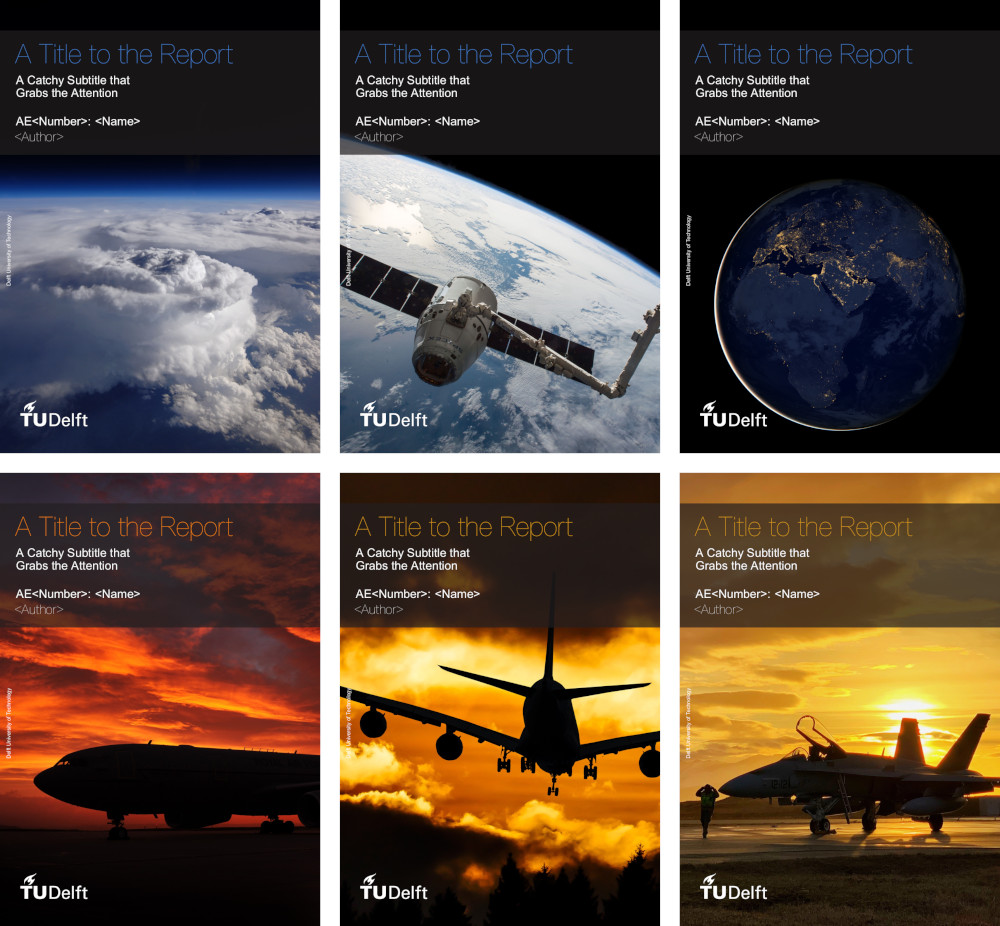
\includegraphics[width=0.75\linewidth]{figures/covers.jpg}
    \caption{Preview of the included cover images}
\end{figure}

\noindent For the first three images, the title color `4884d6' is recommended:

\begin{itemize}
    \item \textbf{cover1.jpg:} Storm Cell Over the Southern Appalachian Mountains by NASA/Stu Broce under CC BY 2.0
    \item \textbf{cover2.jpg:} Canadarm 2 Robotic Arm Grapples SpaceX Dragon by NASA under CC BY-NC 2.0 // Modified
    \item \textbf{cover3.jpg:} City Lights of Africa, Europe, and the Middle East by NASA Earth Observatory under CC BY 2.0
\end{itemize}

\noindent For fourth, the title color `fe860e' is recommended. For the final two, the title color `e3a01b' is recommended:

\begin{itemize}
    \item \textbf{cover4.jpg:} Royal Air Force Voyager Transport Tanker Aircraft by Ministry of Defense/Cpl Ashley Keates under OGL v1.0
    \item \textbf{cover5.jpg:} Aircraft Flying in the Sunset by Gerhard Gellinger
    \item \textbf{cover6.jpg:} F18 at Bodo Air Base Norway by Ministerio de Defensa España under CC BY-NC 2.0
\end{itemize}


%\chapter{Title}
%\label{chapter:title}


%\chapter{Title}
%\label{chapter:title}


%\input{chapter-5} % Create file to add

\chapter{Conclusion}
\label{chapter:conclusion}

A conclusion.


%% Bibliography is numeric style
\printbibliography[title=References] 
\addcontentsline{toc}{chapter}{References}

%% Using letters for chapters
\appendix

\chapter{Title}
\label{appendix:title}


%\chapter{Title}
%\label{appendix:title}


%\input{appendix-c} % Create file to add

\chapter{Task Division}

\setlength\extrarowheight{4pt}
\begin{table}[H]
    \centering
    \caption{Distribution of the workload}
    \label{tab:contr-c2}
    \begin{tabularx}{\textwidth}{lXX}
        \toprule
        & Task & Student Name(s) \\
        \midrule
        & Summary & \\
        Chapter 1 & Introduction &  \\
        Chapter 2 &  & \\
        Chapter 3 &  & \\
        Chapter * &  & \\
        Chapter * & Conclusion &  \\
        \midrule
        & Editors & \\
        & CAD and Figures & \\
        & Document Design and Layout & \\
        \bottomrule
    \end{tabularx}
\end{table}


\end{document}